%!TEX root = ../template.tex
%%%%%%%%%%%%%%%%%%%%%%%%%%%%%%%%%%%%%%%%%%%%%%%%%%%%%%%%%%%%%%%%%%%%
%% chapter3.tex
%% NOVA thesis document file
%%
%% Chapter with a short latex tutorial and examples
%%%%%%%%%%%%%%%%%%%%%%%%%%%%%%%%%%%%%%%%%%%%%%%%%%%%%%%%%%%%%%%%%%%%

\typeout{NT FILE chapter3.tex}%

\makeatletter
\newcommand{\ntifpkgloaded}{%
  \@ifpackageloaded%
}
\makeatother


\chapter{System Model \& Software Architecture}\label{cha:system_model}

This chapter provides an in-depth exploration of the system model and software architecture of TTT.\@ We begin by introducing the system's overarching objectives and foundational principles. Next, we define the design goals that guided its development, followed by a detailed exposition of the system model and software architecture. Subsequently, we present the threat model, analyzing the potential threats and adversaries accounted for in TTT's design. Finally, we conclude with a comprehensive summary that synthesizes the key insights discussed throughout the chapter.

\section{TTT Proposal}\label{sec:system_propostal}

As shown previously in \autoref{sec:motivation}, Tor is a widely used anonymity network that provides users privacy and anonymity while browsing the internet. However, advances in machine learning and data analysis have made it possible to de-anonymize Tor users by analyzing their traffic patterns, therefore compromising the privacy and anonymity that Tor aims to provide [REFS AQUI]. 

This can be achieved through some traffic analysis attacks, such as fingerprinting and traffic correlation. As discussed in \autoref{sec:problem}, these traffic analysis attacks represent a significant threat to Tor users' privacy and anonymity, as sophisticated adversaries can use machine learning and artificial intelligence techniques to analyze monitored traffic patterns and de-anonymize users and their browsing activities.

This way, we propose TTT, an extension of Tor source code that includes a differential private scheduler to protect the users' data and prevent de-anonymization attacks. By incorporating Differential Privacy into the Tor network, we have increased the resistance against fingerprinting and correlation attacks. In addition, TTT also introduces a new differential private `Packet Padding Cells' generation mechanisms, which allows hosts to generate additional traffic that can be used to obfuscate the traffic patterns and make it more difficult for adversaries to analyze the traffic.

The main goal is to reinforce Tor's resistance against traffic analysis attacks, specially fingerprinting and correlation, therefore fortifying users' privacy and anonymity, and ensuring that the solution maintains reasonable performance and usability. To achieve this goal, we designed TTT with the following design goals in mind:
\paragraph{Privacy and Anonymity:} The solution must reinforce Tor's resistance against traffic analysis attacks, specifically fingerprinting and correlation attacks. 
\paragraph{Formally Proven:} The solution must be formally proven to provide a certain level of privacy, by using Differential Privacy. This way, we add a new and important layer of security and trust to the Tor network and users.
\paragraph{Tor's Extension:} The solution must be an extension of the Tor project, respecting Tor's design principles and rules. As a very popular open source project, Tor has a large community of users and developers, and it is important to ensure that the solution can be easily integrated into the existing Tor source code. The project contains a set of principles and rules that we must respect.
\paragraph{Compactibility:} The solution must be easily integrated into the existing Tor network, allowing users and hosts to configure the trade-offs between privacy and performance. The Tor network is composed of several voluntary relays, where hosts decide how to configure. Therefore, we must ensure that the solution can be easily integrated into the existing Tor network and compactible with relays that may be unaware of our solution.
\paragraph{Unobservability:} The solution must enhance Tor's resistance against traffic analysis attacks, specifically fingerprinting and correlation attacks, in comparison to the existing Tor network. 
\paragraph{Configurability:} As an extension of the Tor project, the solution must use the existing Tor configuration files and allow users and hosts to configure the trade-offs between privacy and performance. This way, users can choose the level of privacy they want to achieve.
\paragraph{Performance:} We consider that performance is a key aspect of the solution. However, the solution does not aim to improve the performance of the Tor network, but rather to ensure that the solution does not significantly impact the performance of the Tor network. 

\section{System Model}\label{sec:system_model}

As stated previously, the solution is an extension of the Tor project, so the system model is also similar to the Tor system model, as briefly explained in Section~\ref{sec:tor_network}. In order to preserve the Tor network's design principles and rules, our system model does not introduce any new components or mechanisms in the network layer of the system, as illustrated in~\autoref{fig:system_model}. 

\begin{figure}[!h]
  \centering
  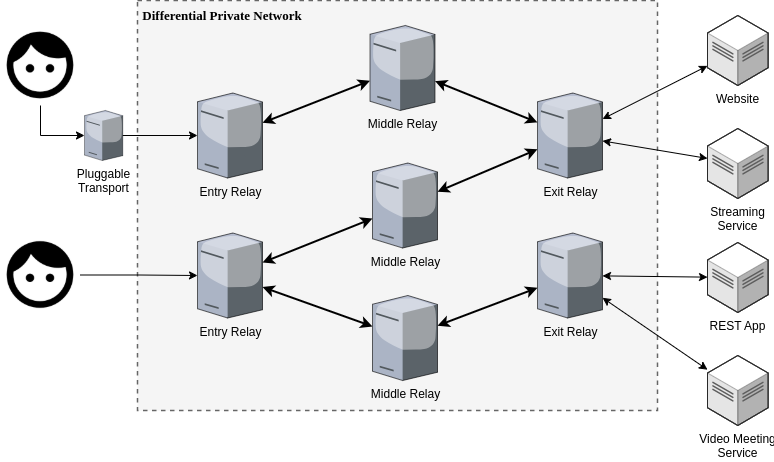
\includegraphics[width=\textwidth]{Chapters/Figures/System_Model_Geral.png}
  \caption{Differential Private Network System Model}\label{fig:system_model}
\end{figure}

Instead, it focuses on enhancing the scheduling on existing Tor relays, with the proposed Differential Privacy Tor Cell Scheduler, and on introducing a new mechanism for generating additional traffic, called `Packet Padding Cells' mechanism, which are both presented further below.

\paragraph{Differential Private Tor Cell Scheduler:} A new scheduler for Tor cells that incorporates Differential Privacy techniques to apply jitter to the Tor network traffic, by applying, or not, a delay on the decision of when the scheduler will run again. Tor's schedulers run on a fix and predetermined time. By setting a random delay on the decision of when the scheduler will run again, we can therefore apply jitter to the Tor network traffic, making it more difficult for adversaries to analyze the traffic patterns and de-anonymize users. As each scheduler can or not apply a delay, the jitter is applied by each individual relay and/or client, making the differential privacy properties accumulate across the network, therefore providing a stronger privacy guarantee. Additionally, this property of the scheduler allows the network to be composed by nodes that are unaware of the solution.
\paragraph{Packet Padding Cells (PPC):} A new mechanism for generating additional traffic. The Tor cells are generated based on a decision-making differential private mechanism triggered when the relay receives a new Tor `relay' cell. The newly generated cells are added to the circuit cell queue of the original cell, which leads to the generated traffic to only be added to active and established circuits.  In comparison to the above scheduler, the differential private properties do not accumulate across the network, as the cells are generated only when a new Tor cell is received, and discarded on reception. This way, considering that 2 segments of the network have senders enhanced with our proposed PPC mechanism, these 2 segments will have a different number of TLS packets and/or different sized TLS packets, making more difficult for adversaries to correlate both segments. Additionally, the client does not produce any additional traffic, unlike the scheduler.

These two new features are designed to work independently, meaning that the user can choose to use one or both of them, but with the same goal of enhancing the Tor network's resistance against traffic analysis attacks.


\section{Threat Model}\label{sec:threat_model}

As mentioned earlier, Tor network is widely used anonymity network that may be vulnerable to traffic analysis attacks, such as fingerprinting and traffic correlation. With these types of attacks, adversaries analyze and monitor traffic in certain segments of the network, aiming to gather information to train and strengthen their machine and deep learning models, which can then be used to de-anonymize users and expose their browsing activities. This way, users that browse the internet through the Tor network, to protect their anonymity, privacy and security, may be vulnerable to these attacks, which can lead to the exposure of their browsing activities and identities, and making Tor inefficient. 

TTT is designed to strengthen the Tor network's privacy protections and bolster its defenses against traffic analysis attacks, with a particular focus on the before mentioned threats. In shaping our threat model, we closely follow the foundational Tor threat model outlined by~\cite{dingledine2004tor}. Accordingly, we consider adversaries who can monitor portions of network traffic, manipulate data flows, operate their own onion routers, and compromise a fraction of existing routers. The adversary's ultimate objective is the de-anonymization of users and the exposure of their browsing activities.

Before defining our adversary model, we first clarify the types of adversaries considered and which are not included in our threat model. State-Level adversaries (SLAd) are capable of observing Tor's traffic patterns in one or few Autonomous Systems (AS). Large-Scope adversaries (LSAd) are considered a group of SLAd that can monitor a significant fraction of the network, by collaborating and working together and therefore controlling the collection of regions controlled by each collaborator. Finally, Omnipresent adversaries (OPAd) are a powerful attacker, or a group of attackers, that can monitor the entire Tor network, including all segments and regions, and therefore can observe all traffic patterns.

\begin{figure}[!h]
  \centering
  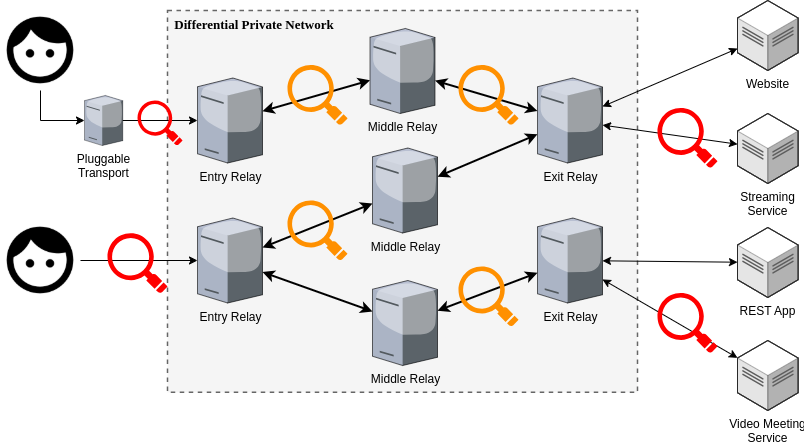
\includegraphics[width=\textwidth]{Chapters/Figures/Threat_Model.png}
  \caption{Threat Model over System Model}\label{fig:thread_model}
\end{figure}

\autoref{fig:thread_model} illustrates the threat model over the system model, showing the adversaries' capabilities and the Tor network segments that they can monitor. The red magnifying glasses indicate the more commonly observed segments of the network, whilst the orange magnifying glasses represent the segments that are less commonly observed. Nonetheless, it is important to note that the adversaries considered by our threat model are not limited to the firstly described segments and our adversaries can monitor any pair of segments in the network.  

For the scope of our solution, we considered SLAd to be the main adversary, as they are more common and realistic in the context of Tor. LSAd are also considered to be a threat and also included in the scope of our threat model, even though we recognize that they are less common. On the other hand, OPAd are not considered in our threat model, as we consider they are not realistic and do not represent a common threat to Tor users.

Building on the original assumptions put forth by~\citeauthor{dingledine2004tor}~\cite{dingledine2004tor}, we consider both passive and active adversaries. A passive adversary merely observes traffic patterns, applying machine learning and data analysis techniques to infer user identities and behaviors. Conversely, an active adversary compromises onion routers to inject traffic into the network — not merely to observe, but to facilitate more sophisticated traffic analysis attacks. Traffic injection, in this context, becomes a strategic tool for the adversary to train machine learning models capable of uncovering users' identities and tracking their navigation through the Tor network. However, it is important to note that we do not take relay compromise into account. In some context, adversaries may deploy a malicious voluntary relay and our solution is not intended to defend users, as the attacker would be able to monitor the traffic patterns and defeat the Packet Padding Cells mechanism. 


In summary, our threat model considers powerful State-Level and Large-Scope adversaries capable of monitoring significant portions of the Tor network traffic, but not on its entirety. These adversaries are equipped with advanced and state-of-the-art machine and deep learning and data analysis techniques. These adversaries may be passive, observing traffic patterns, or active by injecting traffic into the network to train their machine learning models. 


\section{Software Architecture}\label{sec:software_architecture}

To ensure a clear understanding of the software architecture of TTT, we will first present the Tor relay architecture, which is the foundation of TTT, and then we will present the TTT architecture, as an extension of the Tor relay architecture.

\subsection{Tor Relay Architecture}\label{sec:tor_relay_architecture}
Tor relays are the backbone of the Tor network, responsible for routing traffic between clients and servers while maintaining user anonymity.  As explained in more detailed in~\autoref{sec:tor_network}, Tor relays are connected through TCP over TLS connections, forming a network of relays that route TLS packets composed by a variable number of cells between clients, relays and servers, encrypting and decrypting the traffic at each hop, layer by layer.

Our solution extends the Tor relay architecture by introducing a new scheduler and a new mechanism for generating additional traffic, presented in~\autoref{sec:system_model}. 
At the time we proposed, Tor has 2 types of schedulers: the `KIST' scheduler, briefly presented in~\autoref{subsubsec:kist}, which also has a `Lite-KIST' variant for low-end devices, and the Vanilla scheduler, which is a simpler scheduler. To develop our solution, we chose to extend the Vanilla scheduler, as it is simpler and easier to understand, and therefore easier to extend.

\begin{figure}[!h]
  \centering
  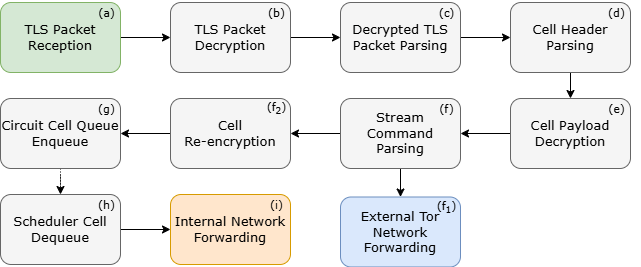
\includegraphics[width=\textwidth]{Chapters/Figures/Tor_Cell_Pipeline.png}
  \caption{Original Cell Processing Pipeline}\label{fig:tor_cell_lifetime}
\end{figure}

To ease the understanding of the Tor relay architecture, we present an  illustration of the lifetime of a Tor cell in a Tor relay in~\autoref{fig:tor_cell_lifetime}. As shown in the figure, after receiving a TLS packet (\(a\)), it gets decrypted (\(b\)) and all Tor Cells within the packet are extracted (\(c\)). For each Tor Cell within the packet, its header is checked (\(d\))  and its payload gets decrypted (\(e\)). After decrypting the payload, the cell's `stream command' is used to determine if the relay is the exit and the cell must be forwards to the destination (\(f_1\)), or if the relay corresponds to an entry or middle relay, in which case the cell is forwarded to the next hop. Finally, the cells that must be forwarded are re-encrypted (\(f_2\)) and enqueued in the respective circuit cell queue (\(g\)). The scheduler then dequeues the cells from the circuit cell queue (\(h\)), and forwards them to the next hop (\(i\)). This process is repeated until the cell reaches its destination, which can be a client or a server. 


\subsection{TTT Architecture}\label{sec:ttt_architecture}

After presenting the Tor relay architecture, together with a better understanding of the Tor cell lifetime in a relay, we can now present the TTT architecture. As stated in~\autoref{sec:system_model}, our solution brings 2 main features to the Tor project: a new scheduler that applies jitter to the Tor network traffic, and a new mechanism for generation additional traffic.

To allow a better comprehension and comparison to the differences of Tor cells lifetime in the original Tor project and in TTT, we present a similar illustration to~\autoref{fig:tor_cell_lifetime} in~\autoref{fig:ttt_cell_lifetime}. The figure illustrates the lifetime of a Tor cell in a TTT relay, showing the differences introduced by our solution.
\begin{figure}[!h]
  \centering
  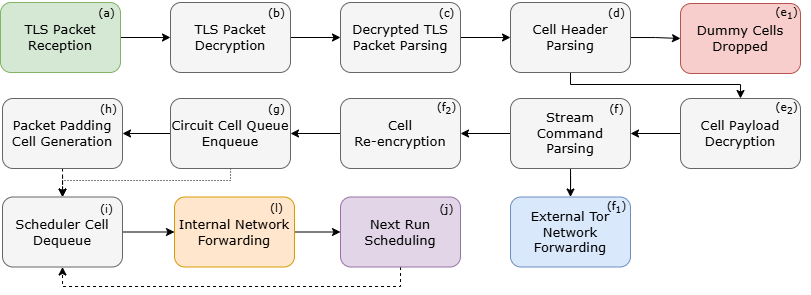
\includegraphics[width=\textwidth]{Chapters/Figures/Solution_Cell_Pipeline.png}
  \caption{TTT Cell Processing Pipeline}\label{fig:ttt_cell_lifetime}
\end{figure}

Upon receiving a TLS packet (\(a\)), the relay decrypts it (\(b\)) and extracts all cells within the packet (\(c\)), same as the original Tor. For each cell within the packet, the relay checks its header (\(d\)). If the cell is a `dummy' cell, it is discarded (\(e_1\)), otherwise the cell is decrypted (\(e_2\)). After decrypting the cell, the `stream command' is checked to determine if the relay is the exit and the cell must be forwarded to the destination (\(f_1\)), or if the relay corresponds to an entry or middle relay, in which case the cell is forwarded to the next hop. For the cells that must be forwarded, they are re-encrypted (\(f_2\)) and enqueued in the respective circuit cell queue (\(g\)). After queuing a cell, the relay decides, based on a differential private algorithm, if it generates a new `Packet Padding Cell' (\(h\)). Newly generated cells are added to the circuit cell queue of the original cell. Once any cell is added to the circuit cell queue, the circuit is marked as `writable', allowing the scheduler to dequeue the cells from the circuit cell queue (\(i\)). After being dequeued cells, the cells are places in the output buffer for retransmission, and forwards the cells to the next hop (\(l\)). Meanwhile, the scheduler calculates if jitter must be applied to the circuit, therefore setting a random delay on the decision of when it will run again or not (\(j\)), impacting the following cells time of retransmission. 

In comparison to the original Tor cell lifetime, the main differences are the step (\(e_1\)), where the dummy cells are discarded, the step (\(i\)), where the process of decision and generation of  Packet Padding Cells take place, and the step (\(m\)), where the scheduler decides if it will apply jitter to the circuit or not. The scheduler implementation of jitter is originated by scheduling the next time the scheduler will run again based on a random delay, which is calculated based on the differential private algorithm. This way, the scheduler can apply jitter to the Tor network traffic and be non-blocking to other relay processes essential for the Tor software to work properly. 

\section{Parameterization}\label{sec:parameterization}

% Explain torrc existence and how it is used to configure the Tor network, and how we use it to configure our solution.

% Explain in more depth the parameterization of the solution, and the main goal of our paramenterizations (paramenters give user control of privacy -> more privacy -> more randomness -> which leads to the need to configure and parameterize algorithms and mechanisms generation of random integers or booleans)

\subsection{Used Techniques}\label{sec:used_techniques}

% To generate pseudo random outcomes -> inspired on DP -> added a library to Tor's source code to generate said numbers and outcomes to be used in the scheduler and Packet Padding Cells generation mechanisms.

% To generate a random number, we need a random number generator
% -> Uniform; Laplace; Poisson; Exponential; Gaussian; Normal

% Add code ?

% To generate or not PPCs, we need a boolean decision generator -> DP Randomized Response

% Insert DPRR Pseudo Code here

\subsection{Jitter Parameterization}\label{sec:jitter_parameterization}

% See notebook

\subsection{Packet Padding Cells Parameterization}\label{sec:packet_padding_parameterization}

% See notebook

\section{Jitter Development Strategy}\label{sec:jitter_development_strategy}

\section{Packet Padding Cells Development Strategy}\label{sec:packet_padding_cells_development_strategy}

\section{Discussion}\label{sec:architeture_discussion}